\documentclass[10pt,twocolumn]{article}
\usepackage[margin=0.75in]{geometry}
\usepackage{amsmath,amssymb}
\usepackage{graphicx}
\usepackage{booktabs}
\usepackage{xcolor}
\usepackage[hidelinks]{hyperref}
\usepackage{caption}
\captionsetup{font=small}
\setlength{\columnsep}{0.25in}
\newcommand{\PropFone}{0.61}
\newcommand{\LRFone}{0.66}
\newcommand{\RFFone}{0.64}
\newcommand{\BBFone}{0.58}
\newcommand{\Rho}{2\%}
\newcommand{\SaboArmShare}{92\%}
\newcommand{\SaboLegChange}{94\%}
\newcommand{\SaboArmChange}{54\%}
\newcommand{\SaboGcOcc}{-0.36}
\newcommand{\SaboPadChange}{15\%}
\newcommand{\SaboScaleLo}{0.49}
\newcommand{\SaboScaleHi}{-0.26}
\newcommand{\BBPad}{22\%}
\newcommand{\BBScale}{39\%}
\newcommand{\RhoWeak}{6\%}
\newcommand{\GCArm}{0.29}
\newcommand{\IGStride}{3\%}
\newcommand{\BBArmUp}{11\%}
\newcommand{\RhoNinety}{4\%}
\newcommand{\BBPadRaw}{0.23}
\newcommand{\BBScaleLowRaw}{0.34}
\newcommand{\BBScaleRaw}{0.39}
\newcommand{\CNNFoneLo}{0.54}
\newcommand{\CNNFoneHi}{0.58}
\newcommand{\STFone}{0.60}
\newcommand{\STPad}{34\%}
\newcommand{\STScale}{80\%}
\newcommand{\STGcArm}{0.61}
\newcommand{\STGcStride}{0.76}
\newcommand{\STGcAsym}{0.68}
\newcommand{\STIgArm}{0.22}
\newcommand{\STPadRaw}{0.34}
\newcommand{\STScaleLowRaw}{0.48}
\newcommand{\STScaleRaw}{0.80}
\newcommand{\SeedGC}{0.41}
\newcommand{\SeedIG}{0.75}


\title{\Large Saliency Maps Do Not Explain Parkinson's Gait Models:\\ A Model That Adds Up Measurable Symptoms Instead}
\author{ParkinsonXAI project \\ \small Draft, November 2026 --- proof of concept, not peer reviewed}
\date{}

\begin{document}
\maketitle

\begin{abstract}
Deep networks can score the severity of Parkinson's disease from walking videos, and heat maps such as
Grad-CAM are often shown as evidence that they look at the right body parts. We test this claim and find it
does not hold. On a public pose-based gait model, Grad-CAM puts \SaboArmShare\ of its weight on the arms,
yet hiding the legs changes \SaboLegChange\ of the predicted grades while hiding the arms changes \SaboArmChange.
The same model also reacts to zero padding and to the overall size of the body. We then propose a model that
is explainable by design. It first measures gait symptoms such as stride length and arm swing with small
differentiable operators. It then turns each measurement into a score contribution through a monotone curve,
and adds a small, penalised unexplained term. On 2953 walks from the CARE-PD dataset the model reaches a
macro-F1 of \PropFone. This is on par with black-box networks (\CNNFoneLo--\STFone) but below logistic regression on
the same features (\LRFone). Its unexplained term carries \Rho\ of the prediction on average. It is unchanged by
padding and body size by construction, while the black boxes change up to \STScale\ of their grades. When we inject a
symptom into healthy walks, its explanation names the injected symptom more often than heat maps do, and, unlike
heat maps, each named contribution is exactly the amount by which the score changed.
\end{abstract}

\section{Motivation}
Parkinson's disease changes how people walk. Steps become shorter, the arms swing less, one side may move less
than the other, and the trunk bends forward. Clinicians score these changes on a 0--4 gait scale; the CARE-PD
benchmark \cite{carepd} provides walks with this score (only 0--3 occur), converted into anonymised 3D body models.

Deep models trained on such data are usually explained after training with saliency methods. We first checked
whether these explanations can be trusted (Fig.~\ref{fig:motivation}). For hand drawings (spirals and waves),
public models reach about 80\% accuracy on spirals, but their Grad-CAM maps fall on the ink strokes barely more
often than a random map and partly survive randomising the network's weights, a failed sanity check
\cite{adebayo2018}. For gait, we used a public spatio-temporal graph network trained to score parkinsonism
\cite{sabo2022}. We found three problems:
\begin{itemize}\setlength\itemsep{1pt}
\item \textbf{The heat map points to the wrong limbs.} Grad-CAM marks the arms, while hiding body parts shows
that the model depends mostly on the legs. Grad-CAM and perturbation-based explanations are negatively
correlated (Spearman $\approx\SaboGcOcc$).
\item \textbf{Padding acts as a shortcut.} Short walks are padded with zero frames. These empty frames receive
up to half of the attribution, and removing the padding changes \SaboPadChange\ of the grades.
\item \textbf{Body size changes the answer.} Rescaling the input skeleton moves the correlation between
predicted and true scores from $+\SaboScaleLo$ to $\SaboScaleHi$.
\end{itemize}
Heat maps also have a deeper limit for movement: the evidence for Parkinson's gait is a property of motion,
such as amplitude, rhythm or symmetry, not a location in an image. We therefore build these properties into
the model.

\begin{figure}[t]
\centering
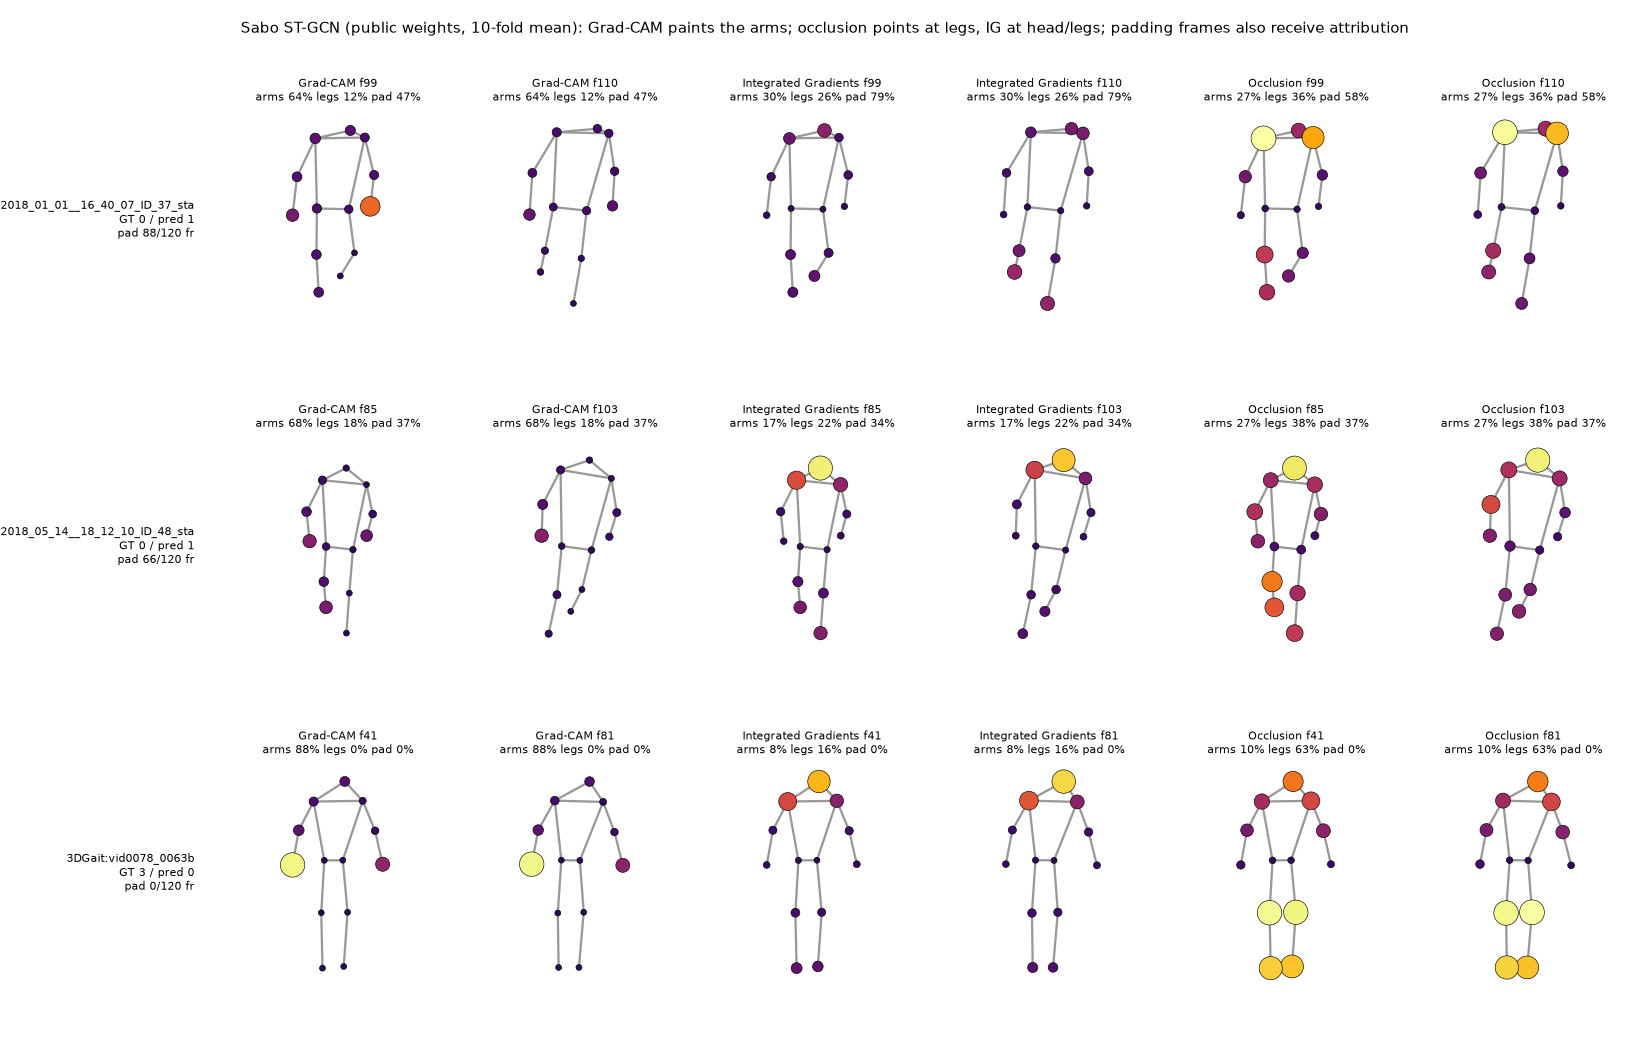
\includegraphics[width=\columnwidth]{figures/sabo_montage.png}
\caption{Public gait model \cite{sabo2022}, mean over 10 cross-validation models. Joint size and colour show
attribution. Grad-CAM (left pair) marks the arms; occlusion (right pair), which measures what the prediction
really depends on, marks the legs. Top two rows: healthy walks wrongly graded 1, with long zero padding.}
\label{fig:motivation}
\end{figure}

\section{Related work}
Concept bottleneck models \cite{koh2020} predict human concepts first and the label from them; later work adds
a residual path and studies how information leaks through it \cite{yuksekgonul2023,havasi2022}. Neural additive
models \cite{agarwal2021} learn one curve per input feature. Learnable signal front ends such as SincNet
\cite{ravanelli2018} learn the parameters of classic filters. Our model combines these ideas for gait: the
concepts are not labelled but computed by differentiable symptom operators, the curves are monotone in a
clinically chosen direction, and the residual is penalised and reported. CARE-PD itself reports a random forest
on handcrafted gait features but no explanation analysis \cite{carepd}. Saliency for time series and skeletons is
known to be fragile \cite{ismail2020,pellano2024}, and tests with known ground truth \cite{zhou2022} motivate our
symptom injection test. We did not find a published model that combines all of these for Parkinson's gait.

\section{Method}
A walk $x$ is a sequence of 13 body joints in 3D at 30 frames per second. Frames that are all zero, such as
padding, are ignored, and every length is divided by the walker's leg length. The model is
\begin{equation}
\hat{s}(x) = b + \sum_{k=1}^{K} e_k(x) + r(x), \quad e_k = g_k\big(c_k(x)\big) - g_k\big(c_k^{\mathrm{ref}}\big).
\label{eq:model}
\end{equation}
Each \emph{symptom operator} $c_k$ measures one property (Table~\ref{tab:ops}). A few of its parameters are
learned, for example the frequency band that defines the step rhythm and the mix of wrist and elbow used for arm
swing. Each \emph{shape function} $g_k$ is a sum of increasing sigmoid curves, multiplied by a fixed clinical
direction (for example, less arm swing can only raise the score). It is therefore monotone by construction.
$c_k^{\mathrm{ref}}$ is the median value in healthy training walks, so $e_k$ reads as ``how much this symptom
raises the score compared with a typical healthy walk''. The residual $r$ is a small convolutional network for
whatever the symptoms miss.

The score is turned into grade probabilities with ordered thresholds $\tau_1<\tau_2$:
\begin{equation}
P(y > j \mid x) = \sigma\big(\hat{s}(x) - \tau_j\big),
\end{equation}
and training minimises the class-weighted negative log-likelihood plus a penalty on the residual,
\begin{equation}
\mathcal{L} = -\log P(y \mid x) + \lambda\, r(x)^2 .
\end{equation}
The explanation is the list of contributions $e_k$ and the residual share
$\rho = |r| / (\sum_k |e_k| + |r|)$, the part of the prediction the symptoms do not explain.

\begin{table}[t]
\centering\small
\begin{tabular}{@{}lll@{}}
\toprule
symptom & how it is measured & direction \\
\midrule
stride length & spread of ankle distance along walking direction & shorter $\uparrow$ \\
cadence & peak of the step-rhythm spectrum (learned band) & learned \\
arm swing & forward swing of wrist/elbow vs shoulder & smaller $\uparrow$ \\
arm asymmetry & $|L-R|/(L+R)$ of arm swing & larger $\uparrow$ \\
rhythm irregularity & entropy of the step-rhythm spectrum & larger $\uparrow$ \\
trunk flexion & forward lean of hip-to-shoulder line & larger $\uparrow$ \\
walking speed & pelvis progress per second & slower $\uparrow$ \\
freezing index & ankle power ratio, high vs low band & larger $\uparrow$ \\
\bottomrule
\end{tabular}
\caption{Symptom operators. All lengths are divided by leg length. $\uparrow$: raises the severity score.}
\label{tab:ops}
\end{table}

\section{Experiments}
\textbf{Data.} We use the four CARE-PD cohorts with gait scores (2953 walks). Score 3 is rare, so we merge
scores 2 and 3 into one class. The 3D joints come from the released body models by forward kinematics.
All models use the same five-fold split, grouped by person so that no walker appears in both training and test,
and stratified by grade (1244, 1071 and 638 walks in grades 0, 1 and 2+). Within each training fold, 10\% of the
people are held out to pick the best epoch. Our model is trained for 40 passes with the Adam optimiser on a
laptop processor in under five minutes in total; the black-box network needs about fifteen minutes on the same
processor. We report accuracy, macro-F1 (the mean of the per-grade F1 scores, which treats rare grades fairly),
the quadratically weighted kappa (which rewards near misses on an ordered scale) and 95\% bootstrap intervals
over walks.

\textbf{Compared models.} (a) A black-box convolutional network over joints and time (temporal convolutions per joint
followed by a layer that mixes joints), trained on 2-second clips of pelvis-centred joints and averaged over each
walk, explained with Grad-CAM and Integrated Gradients; (b) logistic regression and a random forest on the same symptom values (with the
operators fixed at their initial settings), explained by coefficient times change and by TreeSHAP; (c) our model.

\textbf{Symptom injection.} We take every healthy test walk and create three altered copies: arm swing reduced
to 30\%, stride shortened to 55\%, and the left arm's swing reduced to 15\% (asymmetry). We ask two questions:
does the predicted score rise, and does the explanation's largest change point to the injected symptom? For the
black-box network we check whether the joint group with the largest attribution change is the altered one
(arms, legs, or the left arm).

\section{Results}
\begin{table}[t]\centering\small\resizebox{\columnwidth}{!}{%
\begin{tabular}{@{}lccc@{}}\toprule
model & macro-F1 & accuracy & weighted kappa \\ \midrule
Ours: symptom model & 0.61 (0.59--0.63) & 0.62 (0.60--0.64) & 0.62 (0.59--0.64) \\
Logistic regression, same features & 0.66 (0.64--0.68) & 0.67 (0.65--0.68) & 0.65 (0.63--0.68) \\
Random forest, same features & 0.64 (0.62--0.66) & 0.65 (0.63--0.67) & 0.62 (0.60--0.65) \\
Black-box CNN (seed 0) & 0.58 (0.56--0.60) & 0.60 (0.58--0.61) & 0.52 (0.49--0.54) \\
Black-box CNN (seed 1) & 0.54 (0.52--0.56) & 0.58 (0.56--0.59) & 0.47 (0.44--0.49) \\
Black-box CNN (seed 2) & 0.54 (0.52--0.56) & 0.57 (0.56--0.59) & 0.49 (0.46--0.52) \\
Black-box graph network (ST-GCN) & 0.60 (0.58--0.62) & 0.61 (0.59--0.63) & 0.54 (0.52--0.57) \\
Ablation: operators fixed & 0.61 (0.59--0.62) & 0.62 (0.60--0.63) & 0.62 (0.60--0.64) \\
Ablation: no residual & 0.61 (0.59--0.63) & 0.62 (0.60--0.64) & 0.62 (0.60--0.64) \\
Ablation: weak residual penalty & 0.61 (0.59--0.62) & 0.62 (0.60--0.64) & 0.62 (0.60--0.65) \\
\bottomrule\end{tabular}}
\caption{Five-fold, person-grouped results on 2953 CARE-PD walks (grades 0, 1, 2+). Brackets: 95\% bootstrap interval.}
\label{tab:acc}\end{table}

\begin{table}[t]\centering\small\resizebox{\columnwidth}{!}{%
\begin{tabular}{@{}lccc@{}}\toprule
explanation & arm swing & stride & asymmetry \\ \midrule
Ours ($e_k$) & 1.00 / 0.13 & 1.00 / 0.95 & 0.58 / 0.20 \\
Logistic regression & 1.00 / 0.17 & 1.00 / 0.89 & 0.23 / 0.29 \\
Random forest + SHAP & 0.94 / 0.12 & 1.00 / 0.89 & 0.38 / 0.18 \\
CNN + Grad-CAM & 0.29 / 0.11 & 0.60 / 0.75 & 0.17 / 0.05 \\
CNN + Integr. Gradients & 0.19 / 0.11 & 0.03 / 0.75 & 0.20 / 0.05 \\
ST-GCN + Grad-CAM & 0.61 / 0.17 & 0.76 / 0.55 & 0.68 / 0.06 \\
ST-GCN + Integr. Gradients & 0.22 / 0.17 & 0.56 / 0.55 & 0.23 / 0.06 \\
\bottomrule\end{tabular}}
\caption{Symptom injection into all healthy test walks. First number: share of walks where the explanation points at the injected symptom (chance: 0.13 for symptoms, 0.25 or 0.20 for joint groups). Second number: share of walks whose predicted grade went up.}
\label{tab:inj}\end{table}


\textbf{Accuracy (verified).} Table~\ref{tab:acc} shows that our model is about as accurate as the black-box
networks (three seeds of the convolutional network give \CNNFoneLo--\CNNFoneHi; the graph network gives \STFone) but
less accurate than logistic regression on the same gait features. Learning the operator
parameters did not help: freezing them gives almost the same score, and so does removing the residual. A weaker
residual penalty raises the residual share to \RhoWeak\ without improving accuracy. We therefore do not claim an
accuracy gain; the point is that explainability by design costs little compared with a black box.

\textbf{Explanations (verified, with a caveat).} Table~\ref{tab:inj} shows that for reduced arm swing and short
strides our explanation names the injected symptom in every walk. Heat maps depend strongly on the network. For the
convolutional network they point to the altered joints close to chance for arm swing (Grad-CAM \GCArm, chance 0.25),
and Integrated Gradients points to the legs in only \IGStride\ of shortened-stride walks, even though the network does
raise its score for them. For the graph network, Grad-CAM does better (\STGcArm, \STGcStride\ and \STGcAsym), but
here the heat map moves while the decision does not: for asymmetry the grade rises in only 6\% of walks, yet the map
shifts to the left arm in \STGcAsym\ of them. A heat map shows where the input changed, not how much that change
mattered. Heat maps are also unstable across retraining: the same network trained with two seeds gives joint
attributions that agree with a Spearman correlation of only \SeedGC\ for Grad-CAM (\SeedIG\ for Integrated
Gradients). The caveat for our model is important: our operators measure exactly the properties we
inject, so a high hit rate is partly built in. The test shows that the explanation stays honest when the model's
input changes in a known way; it does not show that the operators capture every clinical sign. For asymmetry,
our model splits the change between asymmetry and arm swing, because both measurements move.

\textbf{Robustness (verified).} Adding 60 zero frames or rescaling the body by 0.8 or 1.25 never changed our
model's grade, by construction (Table~\ref{tab:rob}). The convolutional network changed \BBPad\ of grades under
padding and \BBScale\ under a 1.25 scale; the graph network changed \STPad\ and \STScale. A black box could of course be given the same normalisation; the point is that in our
model the protection is part of the structure rather than a preprocessing choice that can be forgotten, as it was
in the public gait model of Section 1.

\begin{table}[t]\centering\small\resizebox{\columnwidth}{!}{%
\begin{tabular}{@{}lccc@{}}\toprule
model & 60 zero frames & body $\times$0.8 & body $\times$1.25 \\ \midrule
Ours & 0.00 & 0.00 & 0.00 \\
Logistic regression & 0.00 & 0.00 & 0.00 \\
Black-box CNN (seed 0) & \BBPadRaw & \BBScaleLowRaw & \BBScaleRaw \\
Black-box graph network & \STPadRaw & \STScaleLowRaw & \STScaleRaw \\
\bottomrule\end{tabular}}
\caption{Share of test walks whose predicted grade changes when 60 empty frames are added at the start or the whole
body is rescaled. Our model and the features are unchanged by construction.}
\label{tab:rob}\end{table}

\textbf{How much is left unexplained (verified).} The residual share $\rho$ has a mean of \Rho\ and a 90th
percentile of \RhoNinety, so almost all of each prediction is carried by named symptoms. Walking speed, stride length,
arm swing and trunk flexion carry most of the weight; the rhythm and freezing terms stay near zero on these short,
straight walks (Fig.~\ref{fig:shape}).

\begin{figure*}[t]
\centering
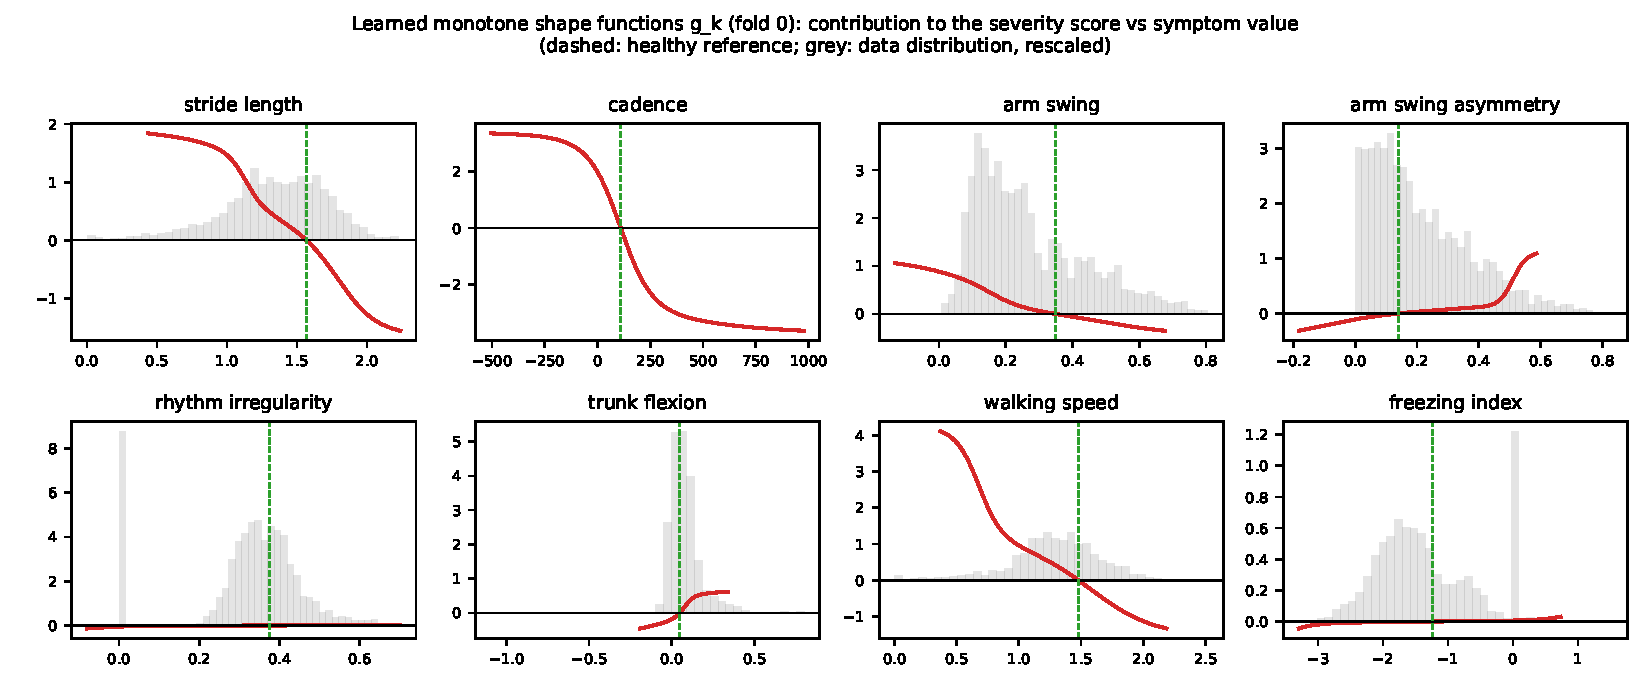
\includegraphics[width=0.92\textwidth]{figures/shape_functions.pdf}
\caption{Learned shape curves (one cross-validation fold). Each panel shows how much one symptom adds to the severity
score compared with a typical healthy walk (dashed line). The direction is fixed by clinical knowledge except for
cadence, whose direction the model learned (fewer steps per minute raises the score).}
\label{fig:shape}
\end{figure*}

\begin{figure}[t]
\centering
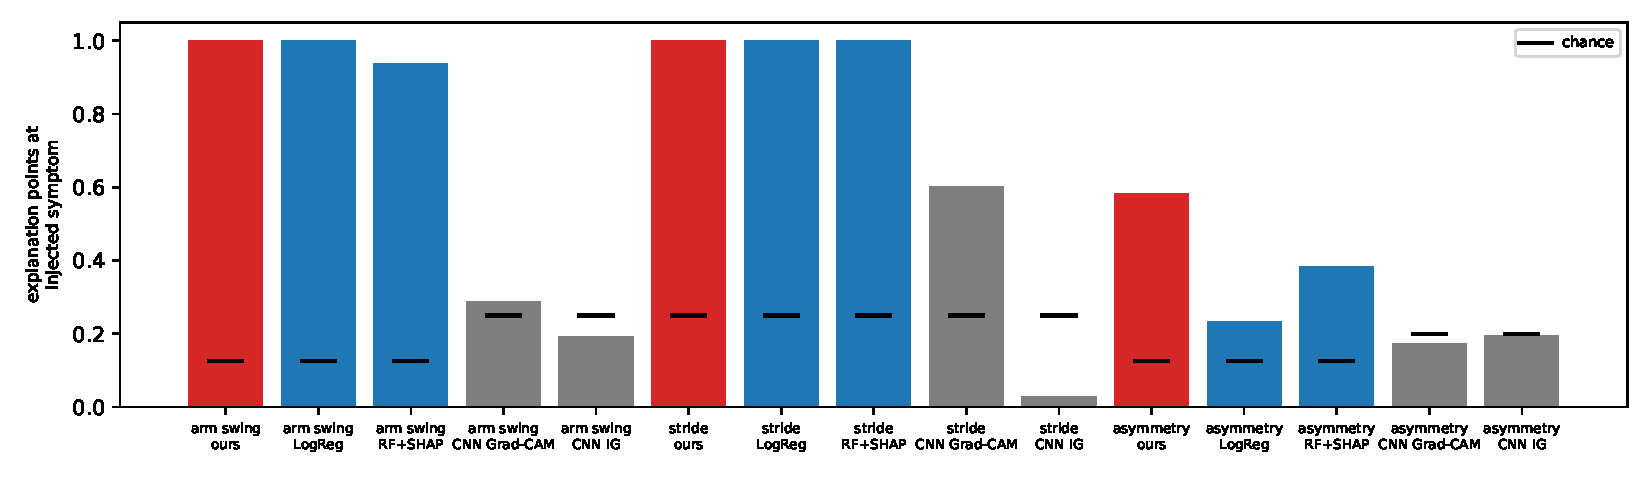
\includegraphics[width=\columnwidth]{figures/injection.pdf}
\caption{Share of injected walks where the explanation points at the injected symptom. Short black lines: chance.}
\label{fig:inj}
\end{figure}

\section{Discussion}
\textbf{What the experiments show.} Three findings are verified on our data. First, post-hoc heat maps of two
different gait networks disagree with perturbation tests about which limbs matter. Second, the networks react to
padding and body size, which a heat map does not reveal. Third, a model built from named symptoms reaches accuracy
between a black box and a linear model, keeps almost all of its prediction in named terms, and its explanation moves
with the injected symptom.

\textbf{What they do not show.} The injection test favours models that measure the injected property, because a
change in arm swing is guaranteed to change the arm swing term. Logistic regression and the random forest on the
same features also do well on two of the three injections, so the advantage comes from the features as much as from
our specific architecture. The test is still informative for the comparison with heat maps: the black-box network did
react to shorter strides, yet Integrated Gradients rarely pointed to the legs. Asymmetry is the hardest case for all
models, because reducing one arm also reduces the average arm swing.

\section{Limitations and next steps}
These are early results on one dataset. The joints come from body-model fits, not from a video pose
detector, so detector noise is missing. The injections are synthetic and simple. The symptom list misses turning
and freezing episodes that need longer recordings. Accuracy is still lower than a linear model on the same
features, which suggests that the learnable operators and the ordinal head need tuning. \emph{Hypotheses not yet
tested:} that clinicians find contribution bars more useful than heat maps, and that the model transfers better
across cohorts. Next steps are leave-one-cohort-out tests, video-based pose input, and a small reader study.

\section{Conclusion}
For Parkinson's gait, popular heat maps can point at the wrong limbs and hide shortcuts. A model that adds up
measured symptoms gives explanations that follow the input by construction, at a modest cost in accuracy.

\small
\bibliographystyle{plain}
\begin{thebibliography}{99}
\bibitem{carepd} V.~Adeli et al. Care-PD: A multi-site anonymized clinical dataset for Parkinson's disease gait assessment. NeurIPS Datasets and Benchmarks, 2025. arXiv:2510.04312.
\bibitem{sabo2022} A.~Sabo et al. Estimating parkinsonism severity in natural gait videos of older adults with dementia. IEEE J. Biomed. Health Inform., 2022. arXiv:2105.03464.
\bibitem{adebayo2018} J.~Adebayo et al. Sanity checks for saliency maps. NeurIPS, 2018.
\bibitem{koh2020} P.~W.~Koh et al. Concept bottleneck models. ICML, 2020.
\bibitem{yuksekgonul2023} M.~Yuksekgonul, M.~Wang, J.~Zou. Post-hoc concept bottleneck models. ICLR, 2023.
\bibitem{havasi2022} M.~Havasi, S.~Parbhoo, F.~Doshi-Velez. Addressing leakage in concept bottleneck models. NeurIPS, 2022.
\bibitem{agarwal2021} R.~Agarwal et al. Neural additive models. NeurIPS, 2021.
\bibitem{ravanelli2018} M.~Ravanelli, Y.~Bengio. Speaker recognition from raw waveform with SincNet. SLT, 2018.
\bibitem{ismail2020} A.~A.~Ismail et al. Benchmarking deep learning interpretability in time series predictions. NeurIPS, 2020.
\bibitem{pellano2024} K.~Pellano, I.~Str\"umke, E.~Ihlen. From movements to metrics: evaluating explainable AI methods in skeleton-based human activity recognition. Sensors, 2024.
\bibitem{zhou2022} Y.~Zhou, S.~Booth, M.~T.~Ribeiro, J.~Shah. Do feature attribution methods correctly attribute features? AAAI, 2022.
\end{thebibliography}
\end{document}
